\documentclass[14pt]{article}
% \usepackage{titling}
\usepackage[utf8]{inputenc}
\usepackage[russian]{babel}
\usepackage[14pt]{extsizes}
\usepackage{graphicx}
\usepackage{tikz}
\usepackage{tikz-feynman}
\usepackage{float}

% \usepackage{titlesec}
\usepackage{amsthm,amsfonts,amsmath,amssymb,amscd, amsbsy}  % Математические дополнения от AMS

\usepackage{url}
\usepackage{listings} 
% \usepackage{cleveref}
\newcommand{\abs}[1]{\lvert#1\rvert}
% \titlelabel{\thetitle.\quad}
\usepackage{geometry}
\geometry{a4paper,top=2.0cm,bottom=2.0cm,left=3.0cm,right=1.5cm,footskip=4mm}
% \setlength{\oddsidemargin}{0cm} % Adjust this value to control the left margin
% \setlength{\textwidth}{17cm}    

\setlength{\droptitle}

\title{Ошибки реализации модели 1 (фон - Пуассоново распределение, эффективность - биномиальное) в TRolke}
\date{}
% \pagenumbering{gobble}


\begin{document}
\maketitle{}
\vspace{-5em} 

\section{Введение}
В статье \cite{Rolke_paper}, описан метод поиска доверительных интервалов методом профилированного правдоподобия.
 Этот метод был реализован в классе TRolke для нескольких моделей описания эффективности регистрации и фона, который, на данный момент, несмотря на признание устаревшим, продолжает использоваться.
 В пункте 2.2 статьи \cite{Rolke_paper} утверждается, что система уравнений для нахождения супремумов, необходимых для поиска интервалов в модели (в TRolke обозначена как модель 1)
$$X\sim Pois(\epsilon \mu +b),\qquad Y\sim Pois(\tau b),\qquad Z\sim Bin(m,\epsilon)$$ 
не может быть решена аналитически, но только численно, что не соответствует действительности.
В ходе реализации численного решения этой системы также был совершен ряд ошибок.

В этом тексте приводится аналитическое решение выше упомянутой системы и реализация этого решения. Проведено сравнение значений супремумов правдоподобия оригинальной реализации (с ошибкой) и исправленной аналитической.
Показано, что аналитическая реализация дает большие значения на множестве параметров, чем супремумы, полученные оригинальным методом.

Также была произведена проверка аналитических решений для остальных моделей --- ошибки в решении уравнений и в реализации нахождения супремумов не были обнаружены.

\section{Существование аналитического решения}

В методе профилированного правдоподобия для построения доверительных интервалов используется следующая статистика:
$$\lambda \left(\mathbf{\pi}_0 | X\right) = \frac{\sup\left\{ L \left(\mathbf{\pi}_0, \mathbf{\theta } | X\right); \mathbf{\theta } \right\} } {\sup\left\{ L \left(\mathbf{\pi}, \mathbf{\theta } | X\right); \mathbf{\pi}, \mathbf{\theta } \right\}} ,$$
где $\mathbf{\theta }$ - ухудшающие параметры.

В модели 1 фон моделируется распределением Пуассона, эффективность --- биномиальным распределением.
$$L(\mu, b, \epsilon | x, y, z, m, \tau) = \frac{\left(\epsilon \mu + b\right)^x}{x!} e^{-\left(\epsilon \mu + b\right)} \frac{\left(\tau b\right)^y}{y!} e^{-\left(\tau b\right)} C_m^z \epsilon^z \left(1 - \epsilon\right)^{m-z} ,$$
$$\ln L(\mu, b, \epsilon | x, y, z, m, \tau) = $$
$$ = x\ln \left(\epsilon \mu + b\right) -\left(\epsilon \mu + b\right) + y\ln \left(\tau b\right) - \tau b + z \ln \epsilon + \left(m - z\right) \ln \left(1 - \epsilon\right) + C ,$$
где $\text{С}$ --- вклад от факториалов и бинома. 
Для нахождения экстремума необходимо решить систему уравнений на частные производные по ухудшающим параметрам. 
В \cite{Rolke_paper} приведена следующая система нелинейных уравнений с утверждением о невозможности получения аналитического решения:
\begin{equation*}
    \frac{\partial }{\partial b}\log l(\mu ,b,\epsilon|x,y,z)=\frac{x}{\epsilon\mu +b}-1+\frac{%
    y}{b}-\tau \doteq 0
\end{equation*}
    
\begin{equation*}
    \frac{\partial }{\partial \epsilon}\log l(\mu ,b,\epsilon|x,y,z)=\frac{x}{\epsilon\mu +b}-\mu +%
    \frac{z}{\epsilon}-\frac{m-z}{1-\epsilon}\doteq 0 .
\end{equation*}

Стоит отметить, что при записи этой системы была совершена опечатка --- потеряна $\mu$ при дифференцировании по $\epsilon$. Корректная система: 
\begin{equation} \label{partial_b_eq}
    \frac{\partial }{\partial b}\log l(\mu ,b,\epsilon|x,y,z)=\frac{x}{\epsilon\mu +b}-1+\frac{%
    y}{b}-\tau \doteq 0
\end{equation}
    
\begin{equation} \label{partial_eff_eq}
    \frac{\partial }{\partial \epsilon}\log l(\mu ,b,\epsilon|x,y,z)=\frac{x \mu}{\epsilon\mu +b}-\mu +%
    \frac{z}{\epsilon}-\frac{m-z}{1-\epsilon}\doteq 0 .
\end{equation}

Вопреки утверждению из статьи \cite{Rolke_paper} эта система уравнений может быть решена аналитически путем сведения системы к уравнению 4-ой степени и использованию соответствующих методов для разрешения оного.
Из уравнения \ref{partial_b_eq} следует, что:
$$\epsilon \mu + b = \frac{x}{1 + \tau - \frac{y}{b}} \Rightarrow \epsilon = \frac{1}{\mu} \left(\frac{x}{1 + \tau - \frac{y}{b}} - b\right) = \frac{b}{\mu} \left( \frac{x - b \left(1 + \tau\right) + y}{b \left(1 + \tau \right) - y}\right) .$$
Введем следующие обозначения: $R(b) = x + y - b \left(1 + \tau\right)$, $Q(b) = b \left(1 + \tau\right) - y$. Отсюда: $\epsilon = \frac{b}{\mu} \frac{R(b)}{Q(b)}$.
Далее путем умножения уравнения \ref{partial_b_eq} на $\mu$  и последующего вычитания из  \ref{partial_eff_eq} получаем:
$$\left(\tau - \frac{y}{b}\right) \mu + \frac{z}{\epsilon} - \frac{m - z}{1 - \epsilon} = 0 \Rightarrow \left(\tau - \frac{y}{b}\right) \mu + z\frac{\mu Q(b)}{b R(b)} - \frac{m - z}{1 - \frac{b}{\mu} \frac{R(b)}{Q(b)}} = 0 .$$
Введем еще одно обозначение $S(b) = \mu Q(b) - b R(b)$. Тогда:

\begin{equation}
\begin{split}
      1 - \frac{b}{\mu} \frac{R(b)}{Q(b)} = \frac{\mu Q(b) - b R(b)}{\mu Q(b)} = \frac{S(b)}{\mu Q(b)} \Rightarrow \\
       \left(\tau - \frac{y}{b}\right) \mu + z\frac{\mu Q(b)}{b R(b)} - \left(m -z\right) \frac{\mu Q(b)}{S(b)} = 0 .
\end{split}
\end{equation}

Умножим это уравнение на $b R(b) S(b)$. Тогда:
$$\left(\tau b - y \right) \mu R(b) S(b) + z \mu Q(b)S(b) - (m-z) \mu b Q(b) R(b) = 0 .$$

Видно, что это уравнение является полиномом 4 степени, которое в общем виде может быть решено аналитически.
%  Путем использования систем компьютерной алгебры 
 Это уравнение может быть приведено к виду
$A b^4 + B b^3 + C b^2 + D b + E =0$, где:
$$A = - \mu \tau \left(1 + \tau\right)^2 ,$$
$$B = \mu (1+\tau) (m (1+\tau)-\mu \tau (1+\tau)+2 \tau x+y+3 \tau y) ,$$ 
$$C = \mu(-m (1+\tau) (x+2 y)-(x+y) (\tau x+2 y+3 \tau y)+\mu (1+\tau) (y+z+\tau (x+3 y+z))) ,$$
$$D = \mu y \left(m (x+y)+(x+y)^2-\mu (x+2 \tau x+2 y+3 \tau y+2 (1+\tau) z)\right) ,$$
$$E = \mu^2 y^2 (x + y + z) .$$

%Примеры решения моего уравнения и изначальной системы из математики 


\section{Ошибка в реализации численного решения}

Из-за утверждения о неразрешимости системы уравнений (\ref{partial_b_eq}, \ref{partial_eff_eq}) в аналитическом виде в TRolke \cite{TRolke, ROOT} был реализован следующий алгоритм нахождения супремумов: %  (если я его правильно понял)
вместо сведения системы к одному уравнению,  выполняется приравнивание полной производной по $\epsilon$ к нулю (расчет этой производной осуществляется методом класса LikeGradMod1) с помощью метода дихотомии (дихотомия реализована в методе класса ProfLikeMod1):
$$\frac{d \ln f}{d \epsilon} = \frac{x}{\epsilon \mu + b} \left(\mu + b^\prime\right) -  \left(\mu + b^\prime\right) + \frac{y}{b} b^\prime - \tau b^\prime + \frac{z}{\epsilon} - \frac{m -z}{1 - \epsilon} = 0 .$$ 
Далее, из исходной системы уравнений (\ref{partial_b_eq}, \ref{partial_eff_eq}) следует, что
$$-\frac{y \mu}{b} +\tau \mu = \frac{m-z}{1-\epsilon} - \frac{z}{\epsilon} .$$
Пусть $\eta = \frac{z}{\epsilon} - \frac{m-z}{1-\epsilon}$, $\eta^\prime = - \frac{z}{\epsilon^2} - \frac{m-z}{\left(1-\epsilon\right)^2}$ тогда  
$$-\frac{y}{b} +\tau = - \frac{\eta}{\mu} \Rightarrow b = \frac{y}{\tau + \eta / \mu} \Rightarrow  b^\prime = - \frac{b^2}{y \mu} \eta^\prime .$$

Но в технической реализации этого уравнения в классе TRolke, представленной на рис. \ref{fig:code_with_error}, указаны следующие $b$ и $b^{\prime}$:
$$b = \frac{y}{\tau - \eta / \mu} , \hspace{1.5cm}  b^\prime = \frac{b^2}{y \mu} \eta^\prime .$$

\begin{figure}[H]
    \centering

    \begin{tikzpicture}
        \node [above right, inner sep=0] (image) at (0,0) {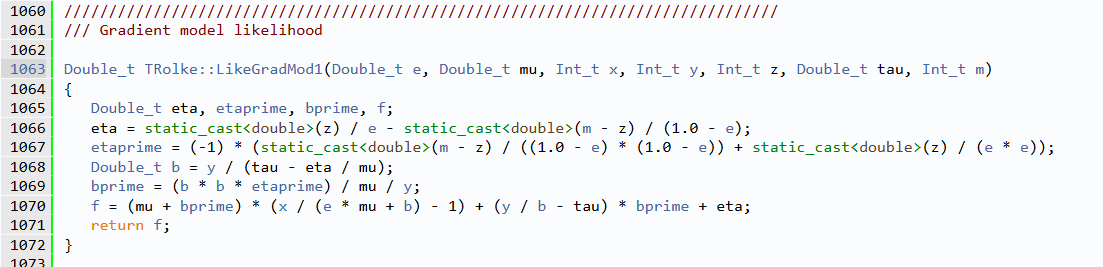
\includegraphics[width=1\textwidth]{graphics/code_with_error.png}};
        \begin{scope} [x={($0.1*(image.south east)$)}, y={($0.1*(image.north west)$)}]


         \draw[line width=0.4mm, red] (0.7, 2.6) rectangle (3.9, 4.1); 
         \draw[red] (3.9, 4.1) ++(0.7, -0.75) node {Ошибка};
         

        \end{scope}
    \end{tikzpicture}
    \caption{Техническая реализация нахождения производной.}
    \label{fig:code_with_error}
\end{figure}


Супремумы, посчитанные этим методом, оказываются меньше супремумов, полученных с использованием аналитического решения, что будет явно показано ниже. 
При исправлении этой ошибки дихотомия находит локальные экстремумы по $\epsilon$, совпадающие с аналитическим решением, но они, в большинстве случаев, не являются искомым супремумом функции правдоподобия.


\section{Реализация исправления ошибки на основе аналитического решения}
Существуют разные методы аналитического решения уравнения 4-ой степени. Было решено использовать метод Феррари из-за относительной простоты записи решения в аналитическом виде (Summary of Ferrari Method в \cite{Eq_solve}).
Реализация метода находится в листинге ниже. С
равнения супремумов для разных параметров представлены на рис.~\ref{fig:Rolke_comparsion_0}, \ref{fig:Rolke_comparsion_1}, \ref{fig:Rolke_comparsion_2} (на всех графиках по оси $y$ отложено $-\sup 2\ln L$ для возможности использования логарифмической шкалы).

\begin{figure}[tbph]
   \centering
   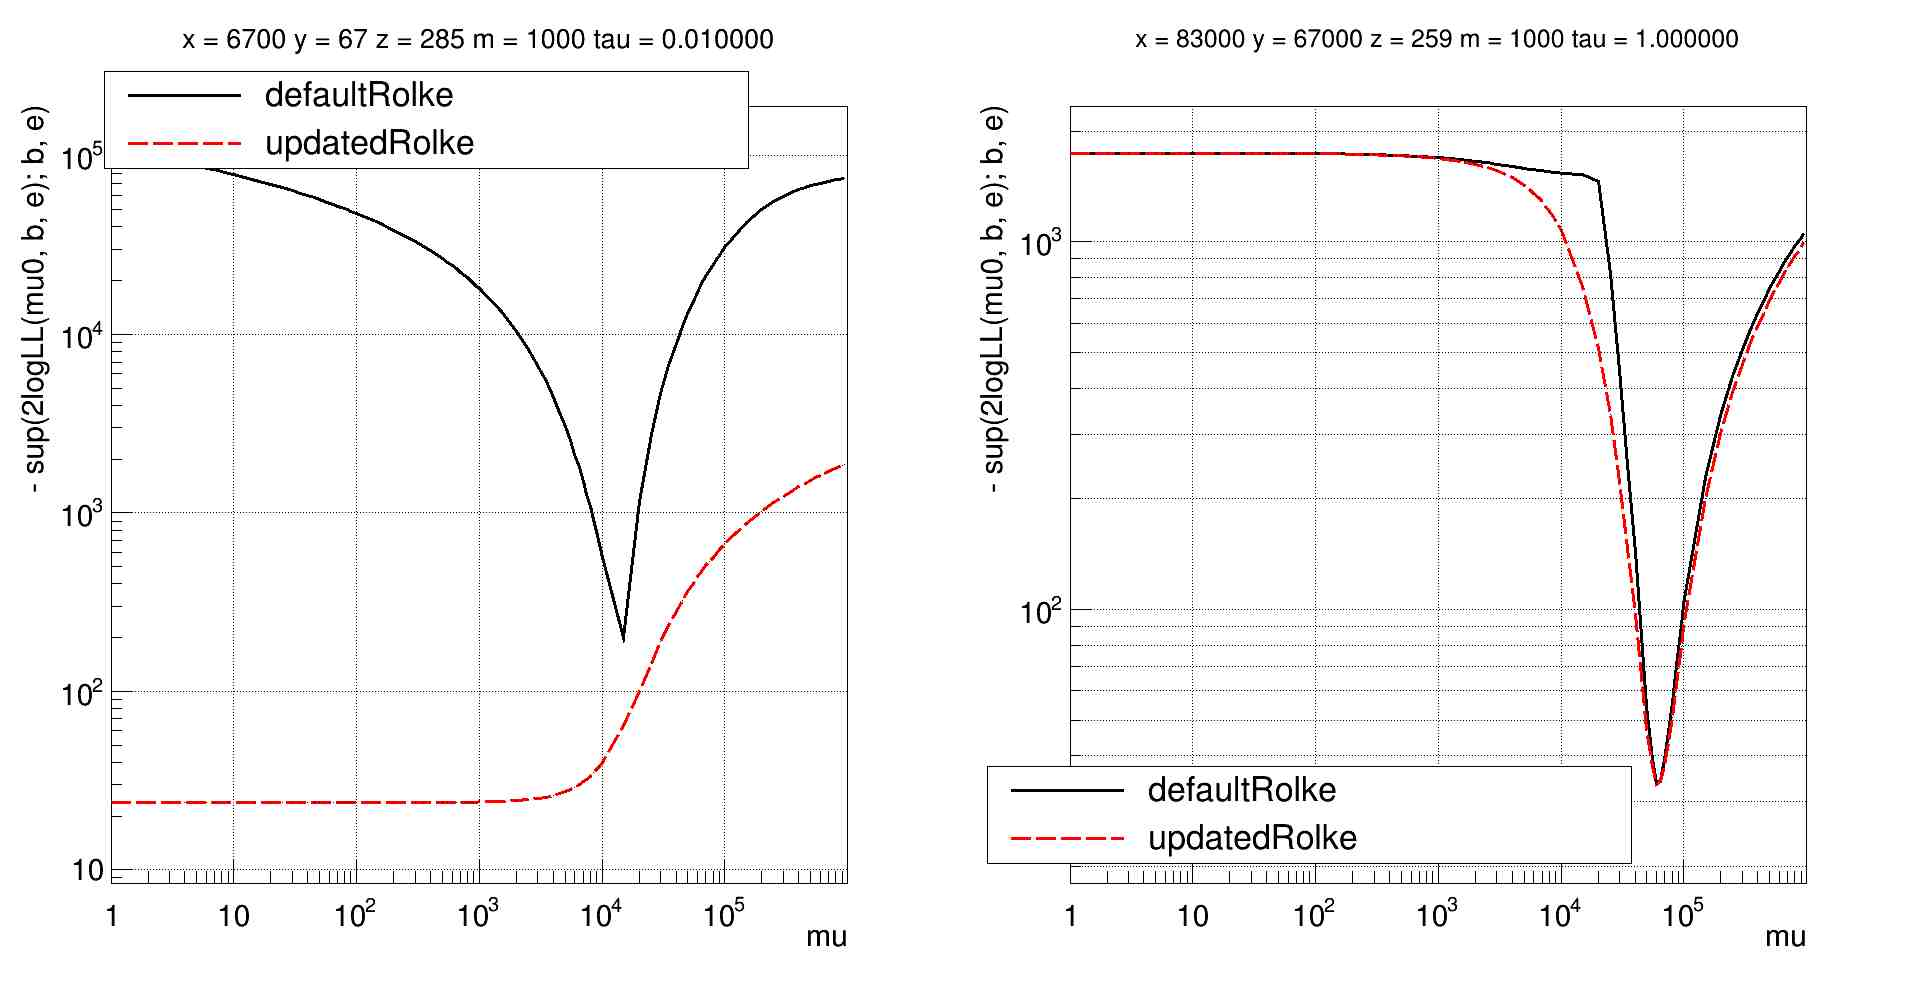
\includegraphics[width=1\textwidth]{graphics/Rolke_comparsion_2_pretty.jpg}
   \caption{Сравнение супремумов, полученных оригинальным и аналитическим методом для разных параметров.}
   \label{fig:Rolke_comparsion_0}
\end{figure}

\begin{figure}[H]
   \centering
   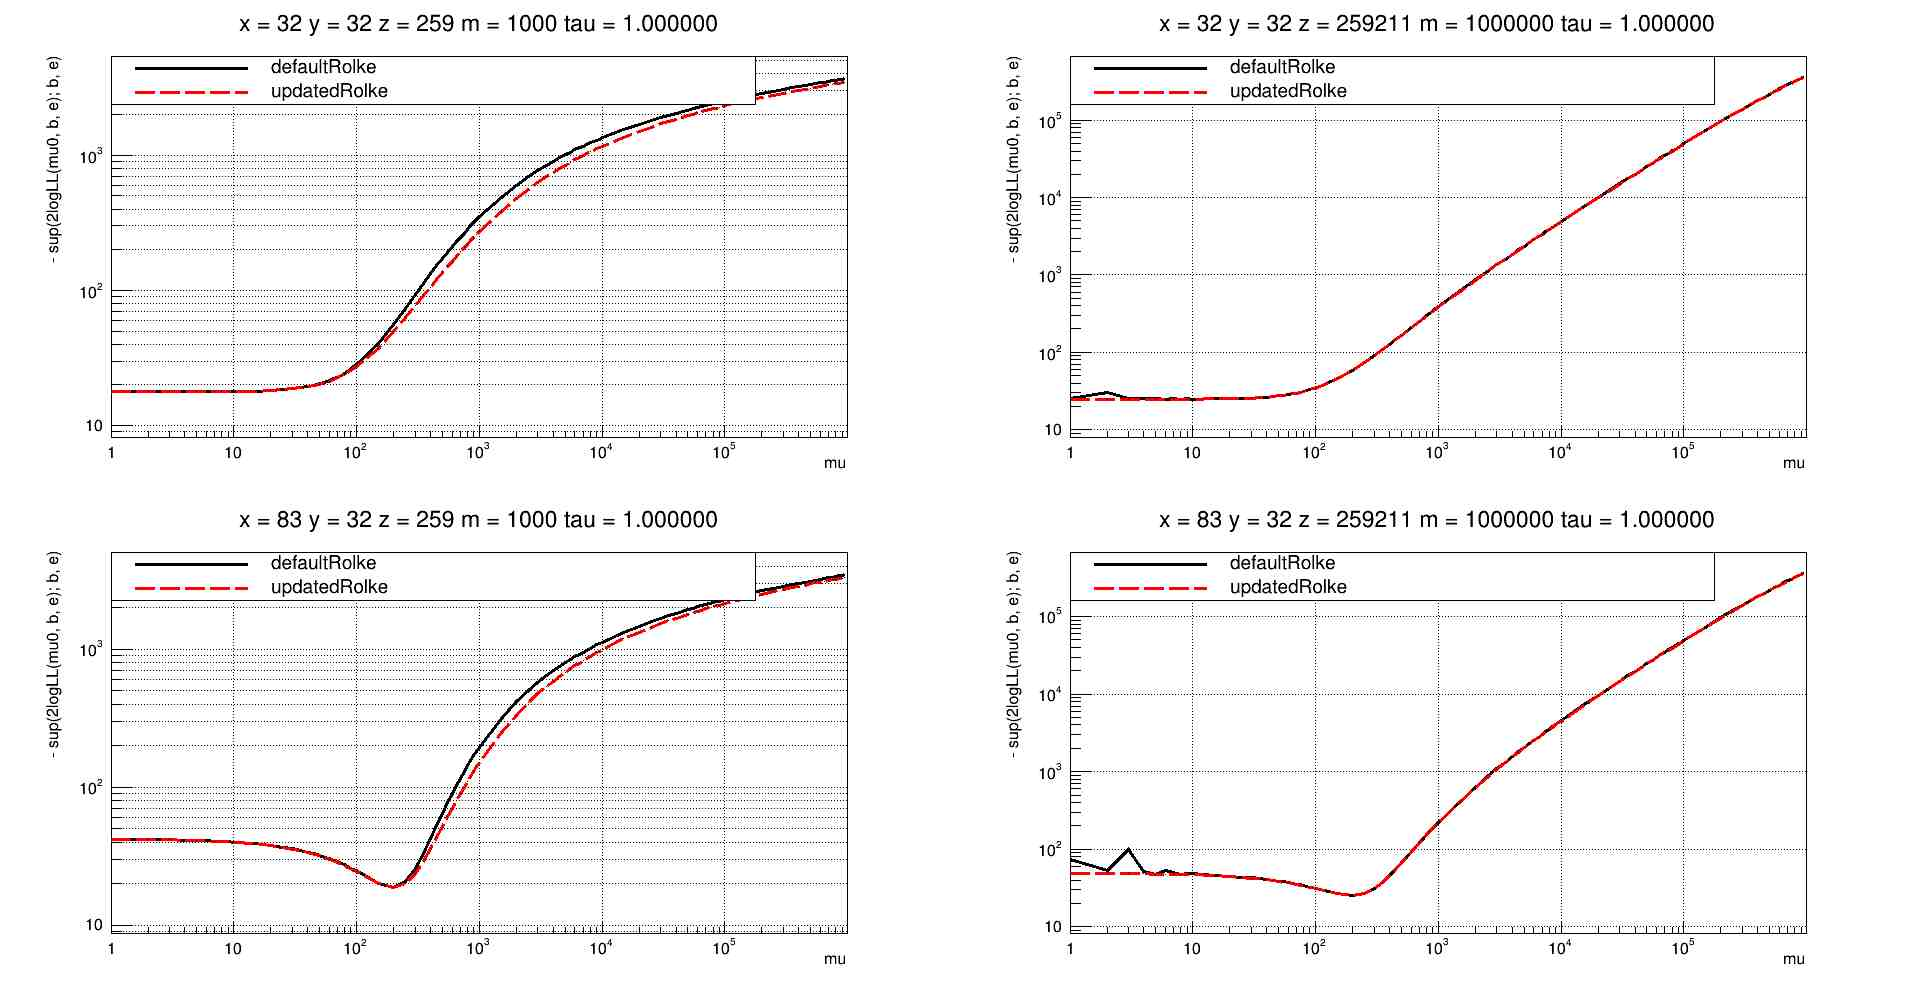
\includegraphics[width=1\textwidth]{graphics/Rolke_comparsion_0_pretty.jpg}
   \caption{Сравнение супремумов, полученных оригинальным и аналитическим методом для разных параметров.}
   \label{fig:Rolke_comparsion_1}
\end{figure}

\begin{figure}[H]
   \centering
   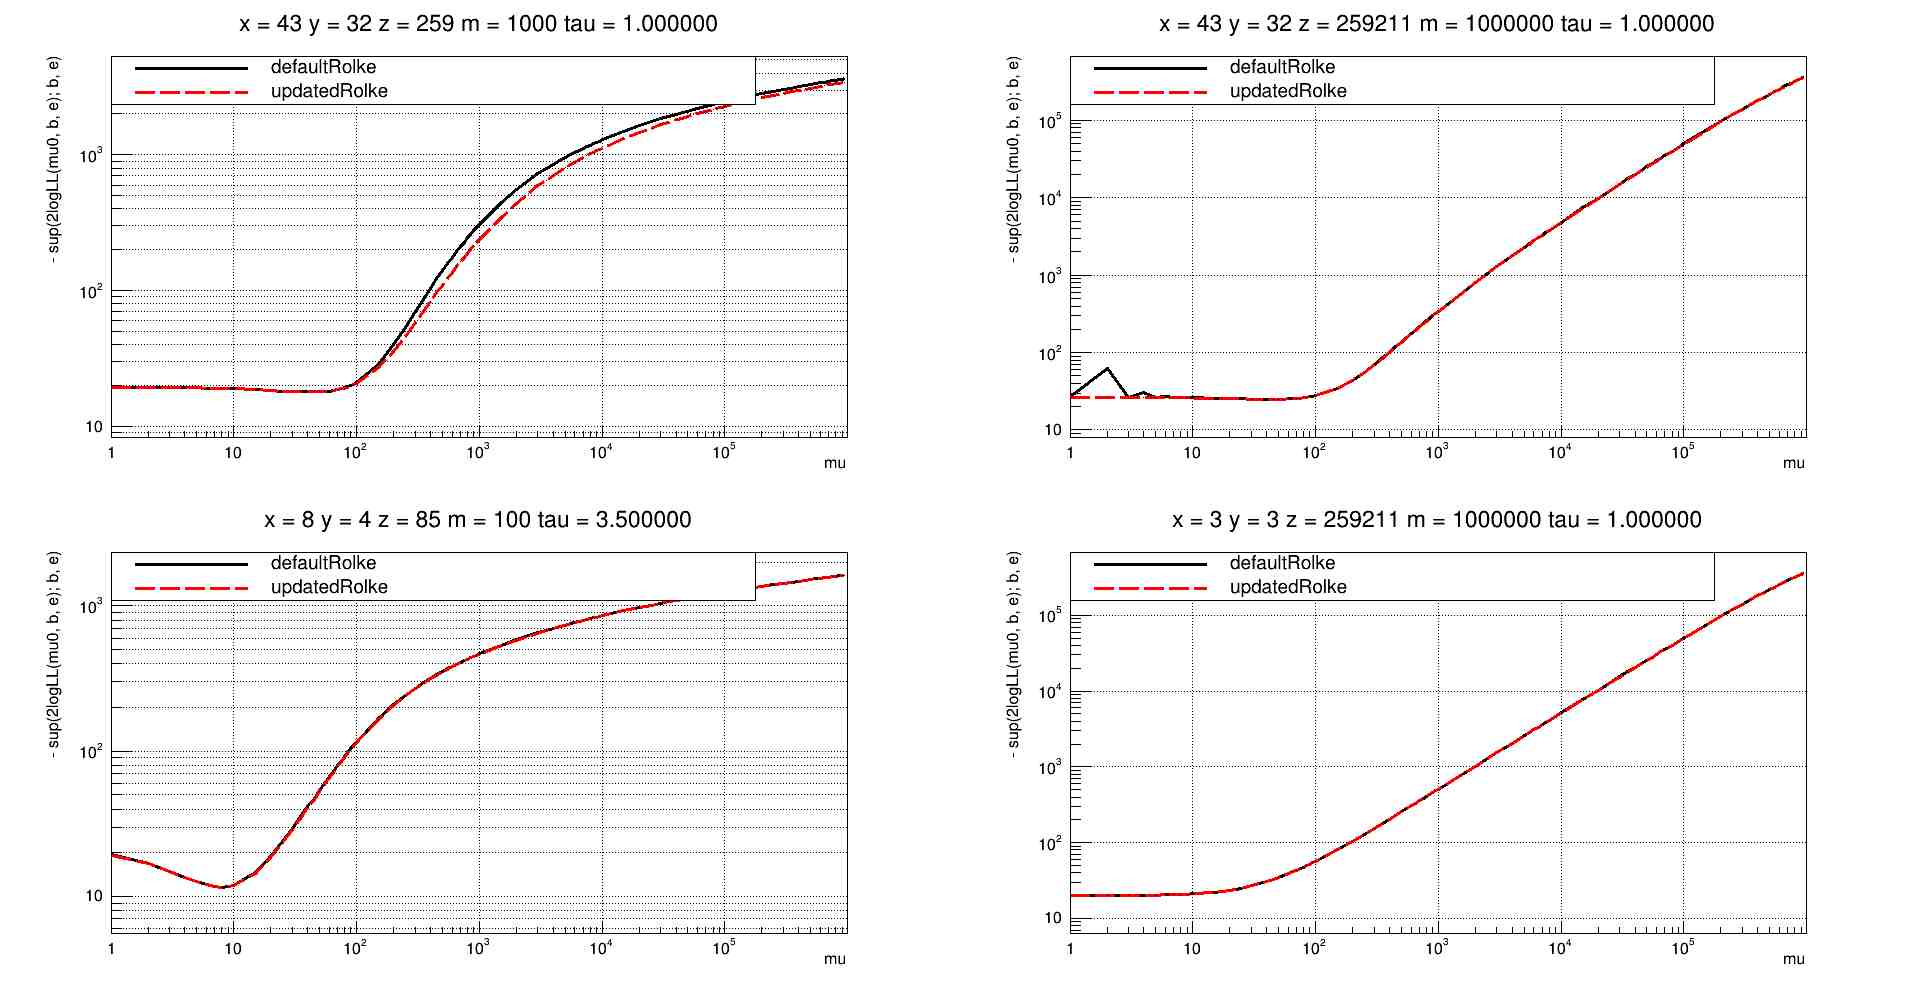
\includegraphics[width=1\textwidth]{graphics/Rolke_comparsion_1_pretty.jpg}
   \caption{Сравнение супремумов, полученных оригинальным и аналитическим методом для разных параметров.}
   \label{fig:Rolke_comparsion_2}
\end{figure}

Видно, что супремумы, полученные аналитически, принимают большие значения, чем супремумы, полученные оригинальным методом. Также стоит отметить отсутствие выбросов у аналитического решения.

\section{Неопределенности в текущем аналитическом решении} 
При некоторых значениях $\mu, x, y, z, m, \tau$ все решения системы могут оказаться в нефизической области. Текущая реализация это не учитывает. Вопрос изменения качества покрытия доверительными интервалами еще не рассмотрен.


\begin{thebibliography}{99}

\bibitem{Rolke_paper}
Rolke W. A., López A. M., Conrad J. Limits and confidence intervals in the presence of nuisance parameters //Nuclear Instruments and Methods in Physics Research Section A:
Accelerators, Spectrometers, Detectors and Associated Equipment. – 2005. – Т. 551. – №. 2-3. – С. 493-503.

\bibitem{TRolke}
Lundberg J. et al. Limits, discovery and cut optimization for a Poisson process with uncertainty in background and signal efficiency: TRolke 2.0 //Computer Physics Communications. – 2010. – Т. 181. – №. 3. – С. 683-686.

\bibitem{ROOT}
ROOT data analysis framework, https://root.cern/, accessed 2021-02-25



\bibitem{Eq_solve}
\url{https://en.wikipedia.org/wiki/Quartic_equation}

\end{thebibliography}

\newpage

\subsection{Листинг кода аналитической реализации поиска супремума}


\begin{lstlisting}[language=C++, basicstyle=\tiny]

void TRolke128_num::ProfLikeMod1Fix(__float128 mu, __float128 &b, __float128 &e, 
      Int_t x, Int_t y, Int_t z, __float128 tau, Int_t m)
{
   __float128 A = - mu * tau * (1.0Q + tau)*(1.0Q + tau);
   __float128 B = mu * (1.0Q + tau) * (- mu * tau * (1.0Q + tau) + 2.0Q * tau * x + y + 
   3.0Q * tau * y + m * (1.0Q + tau));
   __float128 C = mu * (- (x + y) * (tau * x + 2.0Q * y + 3.0Q * tau * y) - 
   m * (1.0Q + tau) * (x + 2.0Q * y) + mu * (1.0Q + tau) * (y + z + tau * (x + 3.0Q * y + z)));
   __float128 D = mu * y * (((__float128) (x + y) * (x + y))  -
    mu * (x + 2.0Q * tau * x + 2.0Q * y + 3.0Q * tau * y + 2.0Q * (1.0Q + tau) * z) + m * (x + y));
   __float128 E = mu * mu * y * y * (x + y + z);

   auto poly4comp = [A, B, C, D, E] (__complex128 b) -> __complex128 {
      __complex128 b_2 = b * b;
      return A * b_2 * b_2 + B * b_2 * b + C * b_2 + D * b + E;
   };

   auto poly4rat = [A, B, C, D, E] (__float128 b) -> __float128 {
      __float128 b_2 = b * b;
      return A * b_2 * b_2 + B * b_2 * b + C * b_2 + D * b + E;
   };

   __float128 A_2 = A * A;
   __float128 B_2 = B * B;

   __float128 alpha = -3.0Q * B_2 / (8.0Q * A_2) + C / A;
   __float128 alpha_2 = alpha * alpha;
   __float128 beta = B_2 * B / (8.0Q * A_2 * A) - B * C / (2.0Q * A_2) + D / A;

   __float128 gamma = - 3.0Q * B_2 * B_2 / (256.0Q * A_2 * A_2) +
    B_2 * C / (16.0Q * A_2 * A) - B * D / (4.0Q * A_2) + E / A; 

   __float128 P = - alpha_2 / 12.0Q - gamma;
   __float128 Q = - alpha_2 * alpha / 108.0Q + alpha * gamma / 3.0Q - beta * beta / 8.0Q;

   __complex128 R = - Q / 2.0Q + csqrtq(Q * Q / 4.0Q + P * P * P / 27.0Q); // taken + sqrt

   __complex128 U = cpowq(R, 1.0Q / 3.0Q);

   __complex128 y_eq =- 5.0Q / 6.0Q * alpha + U - P / (3.0Q * U); // assuming that U !=0;
   __complex128 W = csqrtq(alpha + 2.0Q * y_eq);

   __complex128 back[4]     = {-1.0Q,  -1.0Q, -1.0Q, -1.0Q};
   __complex128 eff[4]      = {10.0Q,  10.0Q, 10.0Q, 10.0Q};
   __float128 minusPlusS[4] = { 1.0Q,   1.0Q, -1.0Q, -1.0Q};
   __float128 minusPlusT[4] = { 1.0Q,  -1.0Q,  1.0Q, -1.0Q};

   __float128 maxLL = (-1.0Q) * FLT128_MAX; 
   __float128 backResult = 0;
   __float128 effResult = 0;

   // loop through signs
   for (int j = 0; j < 4; j ++) {

      back[j] = - B / (4.0Q * A) + (minusPlusS[j] * W + minusPlusT[j] *
       csqrtq(-(3.0Q * alpha + 2.0Q * y_eq + minusPlusS[j] * 2.0Q * beta / W))) / 2.0Q;
      eff[j] = CalcEff(mu, back[j], x, y, z, tau, m);

      __complex128 poly4compVal = poly4comp(back[j]);

      if (crealq(eff[j]) <= 1.0Q && crealq(eff[j]) >= 0.0Q && crealq(back[j]) >= 0.0Q) {
         __float128 currentLL = LikeMod1(mu, crealq(back[j]), crealq(eff[j]), x, y, z, tau, m);
         if (currentLL >= maxLL) {
            backResult = crealq(back[j]);
            effResult = crealq(eff[j]);
            maxLL = currentLL;
            
         } else {
            std::cout << "CurrentLL < maxLL" << std::endl;
         }
         
      } else {
         std::cout << "e or/and b are out of range" << std::endl;
      }

   }

   std::cout << "backResult: " << (double) backResult << " effResult: " << (double) effResult << std::endl;
   b = backResult;
   e = effResult;
}

\end{lstlisting}


\end{document}


